% Plantilla para un Trabajo Fin de Grado de la Universidad de Granada,
% adaptada para el Doble Grado en Ingeniería Informática y Matemáticas.
%
%  Autor: Mario Román.
%  Licencia: GNU GPLv2.
%
% Esta plantilla es una adaptación al castellano de la plantilla
% classicthesis de André Miede, que puede obtenerse en:
%  https://ctan.org/tex-archive/macros/latex/contrib/classicthesis?lang=en
% La plantilla original se licencia en GNU GPLv2.
%
% Esta plantilla usa símbolos de la Universidad de Granada sujetos a la normativa
% de identidad visual corporativa, que puede encontrarse en:
% http://secretariageneral.ugr.es/pages/ivc/normativa
%
% La compilación se realiza con las siguientes instrucciones:
%   pdflatex --shell-escape main.tex
%   bibtex main
%   pdflatex --shell-escape main.tex
%   pdflatex --shell-escape main.tex

% Opciones del tipo de documento
\documentclass[oneside,openright,titlepage,numbers=noenddot,openany,headinclude,footinclude=true,
cleardoublepage=empty,abstractoff,BCOR=5mm,paper=a4,fontsize=12pt,main=spanish]{scrreprt}

% Paquetes de latex que se cargan al inicio. Cubren la entrada de
% texto, gráficos, código fuente y símbolofs.
\usepackage[utf8]{inputenc}
\usepackage[T1]{fontenc}
\usepackage{fixltx2e}
\usepackage{graphicx} % Inclusión de imágenes.
\usepackage{grffile}  % Distintos formatos para imágenes.
\usepackage{longtable} % Tablas multipágina.
\usepackage{wrapfig} % Coloca texto alrededor de una figura.
\usepackage{rotating}
\usepackage[normalem]{ulem}
\usepackage{amsmath}
\usepackage{dsfont}
\usepackage{textcomp}
\usepackage{amssymb}
\usepackage{capt-of}
\usepackage[colorlinks=true]{hyperref}
\usepackage{tikz} % Diagramas conmutativos.
\usepackage{minted} % Código fuente.
\usepackage[T1]{fontenc}
\usepackage[numbers]{natbib}

% Plantilla classicthesis
\usepackage[beramono,eulerchapternumbers,linedheaders,parts,a5paper,dottedtoc,
manychapters,pdfspacing]{classicthesis}

% Geometría y espaciado de párrafos.
\setcounter{secnumdepth}{0}
\usepackage{enumitem}
\setitemize{noitemsep,topsep=0pt,parsep=0pt,partopsep=0pt}
\setlist[enumerate]{topsep=0pt,itemsep=-1ex,partopsep=1ex,parsep=1ex}
\usepackage[top=1in, bottom=1.5in, left=1in, right=1in]{geometry}
\setlength\itemsep{0em}
\setlength{\parindent}{0pt}
\usepackage{parskip}

% Profundidad de la tabla de contenidos.
\setcounter{secnumdepth}{3}

% Usa el paquete minted para mostrar trozos de código.
% Pueden seleccionarse el lenguaje apropiado y el estilo del código.
\usepackage{minted}
\usemintedstyle{colorful}
\setminted{fontsize=\small}
\setminted[haskell]{linenos=false,fontsize=\small}
\renewcommand{\theFancyVerbLine}{\sffamily\textcolor[rgb]{0.5,0.5,1.0}{\oldstylenums{\arabic{FancyVerbLine}}}}

% Path para las imágenes
\graphicspath{{figures/}}

% Archivos de configuración.
%------------------------
% Bibliotecas para matemáticas de latex
%------------------------
\usepackage{amsthm}
\usepackage{amsmath}
\usepackage{tikz}
\usepackage{tikz-cd}
\usetikzlibrary{shapes,fit}
\usepackage{bussproofs}
\EnableBpAbbreviations{}
\usepackage{mathtools}
\usepackage{scalerel}
\usepackage{stmaryrd}

%------------------------
% Estilos para los teoremas
%------------------------
\theoremstyle{plain}
\newtheorem{theorem}{Theorem}
\newtheorem{proposition}{Proposition}
\newtheorem{lemma}{Lemma}
\newtheorem{corollary}{Corollary}

\theoremstyle{definition}
\newtheorem{definition}{Definition}

% Change the proof style so it's in English and add \qed at the end.
\renewenvironment{proof}{{\bfseries Proof.}}{\qed}

\theoremstyle{remark}
\newtheorem{remark}{Remark}
\newtheorem{exampleth}{Example}

% New style for postulates so they are tabulated
\makeatletter
\newtheoremstyle{indented}
	{3pt}% space before
	{3pt}% space after
	{\addtolength{\@totalleftmargin}{3.5em}
		\addtolength{\linewidth}{-3.5em}
		\parshape 1 3.5em \linewidth}% body font
	{}% indent
	{\bfseries}% header font
	{.}% punctuation
	{.5em}% after theorem header
	{}% header specification (empty for default)
\makeatother

% Apply the new style
\theoremstyle{indented}
\newtheorem{postulate}{Postulate}
\newtheorem*{postulate 3'}{Postulate 3'}
\newtheorem*{postulate 2'}{Projective Measurement}

%------------------------
% Macros
% ------------------------

\newcommand*{\B}{\mathbb{B}}
\newcommand*{\C}{\mathds{C}}
\newcommand*{\R}{\mathbb{R}}
\newcommand*{\ra}{\rangle}
\newcommand*{\la}{\langle}

% Para poner sonrisa sobre puntos suspensivos. Uso: \overplace{n}{\dotsc}
\newcommand{\overplace}[2]{%
	\overset{\substack{#1\\\smile}}{#2}%
}  % En macros.tex se almacenan las opciones y comandos para escribir matemáticas.
% ****************************************************************************************************
% classicthesis-config.tex 
% formerly known as loadpackages.sty, classicthesis-ldpkg.sty, and classicthesis-preamble.sty 
% Use it at the beginning of your ClassicThesis.tex, or as a LaTeX Preamble 
% in your ClassicThesis.{tex,lyx} with % ****************************************************************************************************
% classicthesis-config.tex 
% formerly known as loadpackages.sty, classicthesis-ldpkg.sty, and classicthesis-preamble.sty 
% Use it at the beginning of your ClassicThesis.tex, or as a LaTeX Preamble 
% in your ClassicThesis.{tex,lyx} with % ****************************************************************************************************
% classicthesis-config.tex 
% formerly known as loadpackages.sty, classicthesis-ldpkg.sty, and classicthesis-preamble.sty 
% Use it at the beginning of your ClassicThesis.tex, or as a LaTeX Preamble 
% in your ClassicThesis.{tex,lyx} with \input{classicthesis-config}
% ****************************************************************************************************  
% If you like the classicthesis, then I would appreciate a postcard. 
% My address can be found in the file ClassicThesis.pdf. A collection 
% of the postcards I received so far is available online at 
% http://postcards.miede.de
% ****************************************************************************************************


% ****************************************************************************************************
% 0. Set the encoding of your files. UTF-8 is the only sensible encoding nowadays. If you can't read
% äöüßáéçèê∂åëæƒÏ€ then change the encoding setting in your editor, not the line below. If your editor
% does not support utf8 use another editor!
% ****************************************************************************************************
\PassOptionsToPackage{utf8x}{inputenc}
	\usepackage{inputenc}

% ****************************************************************************************************
% 1. Configure classicthesis for your needs here, e.g., remove "drafting" below 
% in order to deactivate the time-stamp on the pages
% ****************************************************************************************************
\PassOptionsToPackage{eulerchapternumbers,listings,drafting,%
		pdfspacing,%floatperchapter,%linedheaders,%
                subfig,beramono,eulermath,parts,dottedtoc}{classicthesis}                                        
% ********************************************************************
% Available options for classicthesis.sty 
% (see ClassicThesis.pdf for more information):
% drafting
% parts nochapters linedheaders
% eulerchapternumbers beramono eulermath pdfspacing minionprospacing
% tocaligned dottedtoc manychapters
% listings floatperchapter subfig
% ********************************************************************

% ****************************************************************************************************
% 2. Personal data and user ad-hoc commands
% ****************************************************************************************************
\newcommand{\myTitle}{A Classic Thesis Style\xspace}
\newcommand{\mySubtitle}{An Homage to The Elements of Typographic Style\xspace}
\newcommand{\myDegree}{Doktor-Ingenieur (Dr.-Ing.)\xspace}
\newcommand{\myName}{André Miede\xspace}
\newcommand{\myProf}{Put name here\xspace}
\newcommand{\myOtherProf}{Put name here\xspace}
\newcommand{\mySupervisor}{Put name here\xspace}
\newcommand{\myFaculty}{Put data here\xspace}
\newcommand{\myDepartment}{Put data here\xspace}
\newcommand{\myUni}{Put data here\xspace}
\newcommand{\myLocation}{Saarbrücken\xspace}
\newcommand{\myTime}{September 2015\xspace}
%\newcommand{\myVersion}{version 4.2\xspace}

% ********************************************************************
% Setup, finetuning, and useful commands
% ********************************************************************
\newcounter{dummy} % necessary for correct hyperlinks (to index, bib, etc.)
\newlength{\abcd} % for ab..z string length calculation
\providecommand{\mLyX}{L\kern-.1667em\lower.25em\hbox{Y}\kern-.125emX\@}
\newcommand{\ie}{i.\,e.}
\newcommand{\Ie}{I.\,e.}
\newcommand{\eg}{e.\,g.}
\newcommand{\Eg}{E.\,g.} 
% ****************************************************************************************************


% ****************************************************************************************************
% 3. Loading some handy packages
% ****************************************************************************************************
% ******************************************************************** 
% Packages with options that might require adjustments
% ******************************************************************** 
%\PassOptionsToPackage{ngerman,american}{babel}   % change this to your language(s)
% Spanish languages need extra options in order to work with this template
% \PassOptionsToPackage{es-lcroman,spanish}{babel}
\usepackage[main=spanish]{babel}

%\usepackage{csquotes}
% \PassOptionsToPackage{%
%     %backend=biber, %instead of bibtex
% 	backend=bibtex8,bibencoding=ascii,%
% 	language=auto,%
% 	style=alpha,%
%     %style=authoryear-comp, % Author 1999, 2010
%     %bibstyle=authoryear,dashed=false, % dashed: substitute rep. author with ---
%     sorting=nyt, % name, year, title
%     maxbibnames=10, % default: 3, et al.
%     %backref=true,%
%     natbib=true % natbib compatibility mode (\citep and \citet still work)
% }{biblatex}
%     \usepackage{biblatex}

% \PassOptionsToPackage{fleqn}{amsmath}       % math environments and more by the AMS 
%     \usepackage{amsmath}

% ******************************************************************** 
% General useful packages
% ******************************************************************** 
\PassOptionsToPackage{T1}{fontenc} % T2A for cyrillics
    \usepackage{fontenc}     
\usepackage{textcomp} % fix warning with missing font shapes
\usepackage{scrhack} % fix warnings when using KOMA with listings package          
\usepackage{xspace} % to get the spacing after macros right  
\usepackage{mparhack} % get marginpar right
\usepackage{fixltx2e} % fixes some LaTeX stuff --> since 2015 in the LaTeX kernel (see below)
%\usepackage[latest]{latexrelease} % will be used once available in more distributions (ISSUE #107)
\PassOptionsToPackage{printonlyused,smaller}{acronym} 
    \usepackage{acronym} % nice macros for handling all acronyms in the thesis
    %\renewcommand{\bflabel}[1]{{#1}\hfill} % fix the list of acronyms --> no longer working
    %\renewcommand*{\acsfont}[1]{\textsc{#1}} 
    \renewcommand*{\aclabelfont}[1]{\acsfont{#1}}
% ****************************************************************************************************


% ****************************************************************************************************
% 4. Setup floats: tables, (sub)figures, and captions
% ****************************************************************************************************
\usepackage{tabularx} % better tables
    \setlength{\extrarowheight}{3pt} % increase table row height
\newcommand{\tableheadline}[1]{\multicolumn{1}{c}{\spacedlowsmallcaps{#1}}}
\newcommand{\myfloatalign}{\centering} % to be used with each float for alignment
\usepackage{caption}
% Thanks to cgnieder and Claus Lahiri
% http://tex.stackexchange.com/questions/69349/spacedlowsmallcaps-in-caption-label
% [REMOVED DUE TO OTHER PROBLEMS, SEE ISSUE #82]    
%\DeclareCaptionLabelFormat{smallcaps}{\bothIfFirst{#1}{~}\MakeTextLowercase{\textsc{#2}}}
%\captionsetup{font=small,labelformat=smallcaps} % format=hang,
\captionsetup{font=small} % format=hang,
\usepackage{subfig}  
% ****************************************************************************************************


% ****************************************************************************************************
% 5. Setup code listings
% ****************************************************************************************************
% \usepackage{listings} 
% %\lstset{emph={trueIndex,root},emphstyle=\color{BlueViolet}}%\underbar} % for special keywords
% \lstset{language={Haskell},morekeywords={PassOptionsToPackage,selectlanguage},keywordstyle=\color{RoyalBlue},basicstyle=\small\ttfamily,commentstyle=\color{Green}\ttfamily,stringstyle=\rmfamily,numbers=none,numberstyle=\scriptsize,stepnumber=5,numbersep=8pt,showstringspaces=false,breaklines=true,belowcaptionskip=.75\baselineskip} 
% ****************************************************************************************************             


% ****************************************************************************************************
% 6. PDFLaTeX, hyperreferences and citation backreferences
% ****************************************************************************************************
% ********************************************************************
% Using PDFLaTeX
% ********************************************************************
\PassOptionsToPackage{pdftex,hyperfootnotes=false,pdfpagelabels}{hyperref}
    \usepackage{hyperref}  % backref linktocpage pagebackref
\pdfcompresslevel=9
\pdfadjustspacing=1 
\PassOptionsToPackage{pdftex}{graphicx}
    \usepackage{graphicx} 
 

% ********************************************************************
% Hyperreferences
% ********************************************************************
\hypersetup{%
    %draft, % = no hyperlinking at all (useful in b/w printouts)
    colorlinks=true, linktocpage=true, pdfstartpage=3, pdfstartview=FitV,%
    % uncomment the following line if you want to have black links (e.g., for printing)
    %colorlinks=false, linktocpage=false, pdfstartpage=3, pdfstartview=FitV, pdfborder={0 0 0},%
    breaklinks=true, pdfpagemode=UseNone, pageanchor=true, pdfpagemode=UseOutlines,%
    plainpages=false, bookmarksnumbered, bookmarksopen=true, bookmarksopenlevel=1,%
    hypertexnames=true, pdfhighlight=/O,%nesting=true,%frenchlinks,%
    urlcolor=webbrown, linkcolor=RoyalBlue, citecolor=webgreen, %pagecolor=RoyalBlue,%
    %urlcolor=Black, linkcolor=Black, citecolor=Black, %pagecolor=Black,%
    pdftitle={\myTitle},%
    pdfauthor={\textcopyright\ \myName, \myUni, \myFaculty},%
    pdfsubject={},%
    pdfkeywords={},%
    pdfcreator={pdfLaTeX},%
    pdfproducer={LaTeX with hyperref and classicthesis}%
}   

% ********************************************************************
% Setup autoreferences
% ********************************************************************
% There are some issues regarding autorefnames
% http://www.ureader.de/msg/136221647.aspx
% http://www.tex.ac.uk/cgi-bin/texfaq2html?label=latexwords
% you have to redefine the makros for the 
% language you use, e.g., american, ngerman
% (as chosen when loading babel/AtBeginDocument)
% ********************************************************************
\makeatletter
\@ifpackageloaded{babel}%
    {%
       \addto\extrasamerican{%
			\renewcommand*{\figureautorefname}{Figure}%
			\renewcommand*{\tableautorefname}{Table}%
			\renewcommand*{\partautorefname}{Part}%
			\renewcommand*{\chapterautorefname}{Chapter}%
			\renewcommand*{\sectionautorefname}{Section}%
			\renewcommand*{\subsectionautorefname}{Section}%
			\renewcommand*{\subsubsectionautorefname}{Section}%     
                }%
       \addto\extrasngerman{% 
			\renewcommand*{\paragraphautorefname}{Absatz}%
			\renewcommand*{\subparagraphautorefname}{Unterabsatz}%
			\renewcommand*{\footnoteautorefname}{Fu\"snote}%
			\renewcommand*{\FancyVerbLineautorefname}{Zeile}%
			\renewcommand*{\theoremautorefname}{Theorem}%
			\renewcommand*{\appendixautorefname}{Anhang}%
			\renewcommand*{\equationautorefname}{Gleichung}%        
			\renewcommand*{\itemautorefname}{Punkt}%
                }%  
            % Fix to getting autorefs for subfigures right (thanks to Belinda Vogt for changing the definition)
            \providecommand{\subfigureautorefname}{\figureautorefname}%             
    }{\relax}
\makeatother


% ****************************************************************************************************
% 7. Last calls before the bar closes
% ****************************************************************************************************
% ********************************************************************
% Development Stuff
% ********************************************************************
\listfiles
%\PassOptionsToPackage{l2tabu,orthodox,abort}{nag}
%   \usepackage{nag}
%\PassOptionsToPackage{warning, all}{onlyamsmath}
%   \usepackage{onlyamsmath}

% ********************************************************************
% Last, but not least...
% ********************************************************************
\usepackage{classicthesis} 
% ****************************************************************************************************


% ****************************************************************************************************
% 8. Further adjustments (experimental)
% ****************************************************************************************************
% ********************************************************************
% Changing the text area
% ********************************************************************
%\linespread{1.05} % a bit more for Palatino
%\areaset[current]{312pt}{761pt} % 686 (factor 2.2) + 33 head + 42 head \the\footskip
%\setlength{\marginparwidth}{7em}%
%\setlength{\marginparsep}{2em}%

% ********************************************************************
% Using different fonts
% ********************************************************************
%\usepackage[oldstylenums]{kpfonts} % oldstyle notextcomp
%\usepackage[osf]{libertine}
%\usepackage[light,condensed,math]{iwona}
%\renewcommand{\sfdefault}{iwona}
%\usepackage{lmodern} % <-- no osf support :-(
%\usepackage{cfr-lm} % 
%\usepackage[urw-garamond]{mathdesign} <-- no osf support :-(
%\usepackage[default,osfigures]{opensans} % scale=0.95 
%\usepackage[sfdefault]{FiraSans}
% ****************************************************************************************************

% ****************************************************************************************************  
% If you like the classicthesis, then I would appreciate a postcard. 
% My address can be found in the file ClassicThesis.pdf. A collection 
% of the postcards I received so far is available online at 
% http://postcards.miede.de
% ****************************************************************************************************


% ****************************************************************************************************
% 0. Set the encoding of your files. UTF-8 is the only sensible encoding nowadays. If you can't read
% äöüßáéçèê∂åëæƒÏ€ then change the encoding setting in your editor, not the line below. If your editor
% does not support utf8 use another editor!
% ****************************************************************************************************
\PassOptionsToPackage{utf8x}{inputenc}
	\usepackage{inputenc}

% ****************************************************************************************************
% 1. Configure classicthesis for your needs here, e.g., remove "drafting" below 
% in order to deactivate the time-stamp on the pages
% ****************************************************************************************************
\PassOptionsToPackage{eulerchapternumbers,listings,drafting,%
		pdfspacing,%floatperchapter,%linedheaders,%
                subfig,beramono,eulermath,parts,dottedtoc}{classicthesis}                                        
% ********************************************************************
% Available options for classicthesis.sty 
% (see ClassicThesis.pdf for more information):
% drafting
% parts nochapters linedheaders
% eulerchapternumbers beramono eulermath pdfspacing minionprospacing
% tocaligned dottedtoc manychapters
% listings floatperchapter subfig
% ********************************************************************

% ****************************************************************************************************
% 2. Personal data and user ad-hoc commands
% ****************************************************************************************************
\newcommand{\myTitle}{A Classic Thesis Style\xspace}
\newcommand{\mySubtitle}{An Homage to The Elements of Typographic Style\xspace}
\newcommand{\myDegree}{Doktor-Ingenieur (Dr.-Ing.)\xspace}
\newcommand{\myName}{André Miede\xspace}
\newcommand{\myProf}{Put name here\xspace}
\newcommand{\myOtherProf}{Put name here\xspace}
\newcommand{\mySupervisor}{Put name here\xspace}
\newcommand{\myFaculty}{Put data here\xspace}
\newcommand{\myDepartment}{Put data here\xspace}
\newcommand{\myUni}{Put data here\xspace}
\newcommand{\myLocation}{Saarbrücken\xspace}
\newcommand{\myTime}{September 2015\xspace}
%\newcommand{\myVersion}{version 4.2\xspace}

% ********************************************************************
% Setup, finetuning, and useful commands
% ********************************************************************
\newcounter{dummy} % necessary for correct hyperlinks (to index, bib, etc.)
\newlength{\abcd} % for ab..z string length calculation
\providecommand{\mLyX}{L\kern-.1667em\lower.25em\hbox{Y}\kern-.125emX\@}
\newcommand{\ie}{i.\,e.}
\newcommand{\Ie}{I.\,e.}
\newcommand{\eg}{e.\,g.}
\newcommand{\Eg}{E.\,g.} 
% ****************************************************************************************************


% ****************************************************************************************************
% 3. Loading some handy packages
% ****************************************************************************************************
% ******************************************************************** 
% Packages with options that might require adjustments
% ******************************************************************** 
%\PassOptionsToPackage{ngerman,american}{babel}   % change this to your language(s)
% Spanish languages need extra options in order to work with this template
% \PassOptionsToPackage{es-lcroman,spanish}{babel}
\usepackage[main=spanish]{babel}

%\usepackage{csquotes}
% \PassOptionsToPackage{%
%     %backend=biber, %instead of bibtex
% 	backend=bibtex8,bibencoding=ascii,%
% 	language=auto,%
% 	style=alpha,%
%     %style=authoryear-comp, % Author 1999, 2010
%     %bibstyle=authoryear,dashed=false, % dashed: substitute rep. author with ---
%     sorting=nyt, % name, year, title
%     maxbibnames=10, % default: 3, et al.
%     %backref=true,%
%     natbib=true % natbib compatibility mode (\citep and \citet still work)
% }{biblatex}
%     \usepackage{biblatex}

% \PassOptionsToPackage{fleqn}{amsmath}       % math environments and more by the AMS 
%     \usepackage{amsmath}

% ******************************************************************** 
% General useful packages
% ******************************************************************** 
\PassOptionsToPackage{T1}{fontenc} % T2A for cyrillics
    \usepackage{fontenc}     
\usepackage{textcomp} % fix warning with missing font shapes
\usepackage{scrhack} % fix warnings when using KOMA with listings package          
\usepackage{xspace} % to get the spacing after macros right  
\usepackage{mparhack} % get marginpar right
\usepackage{fixltx2e} % fixes some LaTeX stuff --> since 2015 in the LaTeX kernel (see below)
%\usepackage[latest]{latexrelease} % will be used once available in more distributions (ISSUE #107)
\PassOptionsToPackage{printonlyused,smaller}{acronym} 
    \usepackage{acronym} % nice macros for handling all acronyms in the thesis
    %\renewcommand{\bflabel}[1]{{#1}\hfill} % fix the list of acronyms --> no longer working
    %\renewcommand*{\acsfont}[1]{\textsc{#1}} 
    \renewcommand*{\aclabelfont}[1]{\acsfont{#1}}
% ****************************************************************************************************


% ****************************************************************************************************
% 4. Setup floats: tables, (sub)figures, and captions
% ****************************************************************************************************
\usepackage{tabularx} % better tables
    \setlength{\extrarowheight}{3pt} % increase table row height
\newcommand{\tableheadline}[1]{\multicolumn{1}{c}{\spacedlowsmallcaps{#1}}}
\newcommand{\myfloatalign}{\centering} % to be used with each float for alignment
\usepackage{caption}
% Thanks to cgnieder and Claus Lahiri
% http://tex.stackexchange.com/questions/69349/spacedlowsmallcaps-in-caption-label
% [REMOVED DUE TO OTHER PROBLEMS, SEE ISSUE #82]    
%\DeclareCaptionLabelFormat{smallcaps}{\bothIfFirst{#1}{~}\MakeTextLowercase{\textsc{#2}}}
%\captionsetup{font=small,labelformat=smallcaps} % format=hang,
\captionsetup{font=small} % format=hang,
\usepackage{subfig}  
% ****************************************************************************************************


% ****************************************************************************************************
% 5. Setup code listings
% ****************************************************************************************************
% \usepackage{listings} 
% %\lstset{emph={trueIndex,root},emphstyle=\color{BlueViolet}}%\underbar} % for special keywords
% \lstset{language={Haskell},morekeywords={PassOptionsToPackage,selectlanguage},keywordstyle=\color{RoyalBlue},basicstyle=\small\ttfamily,commentstyle=\color{Green}\ttfamily,stringstyle=\rmfamily,numbers=none,numberstyle=\scriptsize,stepnumber=5,numbersep=8pt,showstringspaces=false,breaklines=true,belowcaptionskip=.75\baselineskip} 
% ****************************************************************************************************             


% ****************************************************************************************************
% 6. PDFLaTeX, hyperreferences and citation backreferences
% ****************************************************************************************************
% ********************************************************************
% Using PDFLaTeX
% ********************************************************************
\PassOptionsToPackage{pdftex,hyperfootnotes=false,pdfpagelabels}{hyperref}
    \usepackage{hyperref}  % backref linktocpage pagebackref
\pdfcompresslevel=9
\pdfadjustspacing=1 
\PassOptionsToPackage{pdftex}{graphicx}
    \usepackage{graphicx} 
 

% ********************************************************************
% Hyperreferences
% ********************************************************************
\hypersetup{%
    %draft, % = no hyperlinking at all (useful in b/w printouts)
    colorlinks=true, linktocpage=true, pdfstartpage=3, pdfstartview=FitV,%
    % uncomment the following line if you want to have black links (e.g., for printing)
    %colorlinks=false, linktocpage=false, pdfstartpage=3, pdfstartview=FitV, pdfborder={0 0 0},%
    breaklinks=true, pdfpagemode=UseNone, pageanchor=true, pdfpagemode=UseOutlines,%
    plainpages=false, bookmarksnumbered, bookmarksopen=true, bookmarksopenlevel=1,%
    hypertexnames=true, pdfhighlight=/O,%nesting=true,%frenchlinks,%
    urlcolor=webbrown, linkcolor=RoyalBlue, citecolor=webgreen, %pagecolor=RoyalBlue,%
    %urlcolor=Black, linkcolor=Black, citecolor=Black, %pagecolor=Black,%
    pdftitle={\myTitle},%
    pdfauthor={\textcopyright\ \myName, \myUni, \myFaculty},%
    pdfsubject={},%
    pdfkeywords={},%
    pdfcreator={pdfLaTeX},%
    pdfproducer={LaTeX with hyperref and classicthesis}%
}   

% ********************************************************************
% Setup autoreferences
% ********************************************************************
% There are some issues regarding autorefnames
% http://www.ureader.de/msg/136221647.aspx
% http://www.tex.ac.uk/cgi-bin/texfaq2html?label=latexwords
% you have to redefine the makros for the 
% language you use, e.g., american, ngerman
% (as chosen when loading babel/AtBeginDocument)
% ********************************************************************
\makeatletter
\@ifpackageloaded{babel}%
    {%
       \addto\extrasamerican{%
			\renewcommand*{\figureautorefname}{Figure}%
			\renewcommand*{\tableautorefname}{Table}%
			\renewcommand*{\partautorefname}{Part}%
			\renewcommand*{\chapterautorefname}{Chapter}%
			\renewcommand*{\sectionautorefname}{Section}%
			\renewcommand*{\subsectionautorefname}{Section}%
			\renewcommand*{\subsubsectionautorefname}{Section}%     
                }%
       \addto\extrasngerman{% 
			\renewcommand*{\paragraphautorefname}{Absatz}%
			\renewcommand*{\subparagraphautorefname}{Unterabsatz}%
			\renewcommand*{\footnoteautorefname}{Fu\"snote}%
			\renewcommand*{\FancyVerbLineautorefname}{Zeile}%
			\renewcommand*{\theoremautorefname}{Theorem}%
			\renewcommand*{\appendixautorefname}{Anhang}%
			\renewcommand*{\equationautorefname}{Gleichung}%        
			\renewcommand*{\itemautorefname}{Punkt}%
                }%  
            % Fix to getting autorefs for subfigures right (thanks to Belinda Vogt for changing the definition)
            \providecommand{\subfigureautorefname}{\figureautorefname}%             
    }{\relax}
\makeatother


% ****************************************************************************************************
% 7. Last calls before the bar closes
% ****************************************************************************************************
% ********************************************************************
% Development Stuff
% ********************************************************************
\listfiles
%\PassOptionsToPackage{l2tabu,orthodox,abort}{nag}
%   \usepackage{nag}
%\PassOptionsToPackage{warning, all}{onlyamsmath}
%   \usepackage{onlyamsmath}

% ********************************************************************
% Last, but not least...
% ********************************************************************
\usepackage{classicthesis} 
% ****************************************************************************************************


% ****************************************************************************************************
% 8. Further adjustments (experimental)
% ****************************************************************************************************
% ********************************************************************
% Changing the text area
% ********************************************************************
%\linespread{1.05} % a bit more for Palatino
%\areaset[current]{312pt}{761pt} % 686 (factor 2.2) + 33 head + 42 head \the\footskip
%\setlength{\marginparwidth}{7em}%
%\setlength{\marginparsep}{2em}%

% ********************************************************************
% Using different fonts
% ********************************************************************
%\usepackage[oldstylenums]{kpfonts} % oldstyle notextcomp
%\usepackage[osf]{libertine}
%\usepackage[light,condensed,math]{iwona}
%\renewcommand{\sfdefault}{iwona}
%\usepackage{lmodern} % <-- no osf support :-(
%\usepackage{cfr-lm} % 
%\usepackage[urw-garamond]{mathdesign} <-- no osf support :-(
%\usepackage[default,osfigures]{opensans} % scale=0.95 
%\usepackage[sfdefault]{FiraSans}
% ****************************************************************************************************

% ****************************************************************************************************  
% If you like the classicthesis, then I would appreciate a postcard. 
% My address can be found in the file ClassicThesis.pdf. A collection 
% of the postcards I received so far is available online at 
% http://postcards.miede.de
% ****************************************************************************************************


% ****************************************************************************************************
% 0. Set the encoding of your files. UTF-8 is the only sensible encoding nowadays. If you can't read
% äöüßáéçèê∂åëæƒÏ€ then change the encoding setting in your editor, not the line below. If your editor
% does not support utf8 use another editor!
% ****************************************************************************************************
\PassOptionsToPackage{utf8x}{inputenc}
	\usepackage{inputenc}

% ****************************************************************************************************
% 1. Configure classicthesis for your needs here, e.g., remove "drafting" below 
% in order to deactivate the time-stamp on the pages
% ****************************************************************************************************
\PassOptionsToPackage{eulerchapternumbers,listings,drafting,%
		pdfspacing,%floatperchapter,%linedheaders,%
                subfig,beramono,eulermath,parts,dottedtoc}{classicthesis}                                        
% ********************************************************************
% Available options for classicthesis.sty 
% (see ClassicThesis.pdf for more information):
% drafting
% parts nochapters linedheaders
% eulerchapternumbers beramono eulermath pdfspacing minionprospacing
% tocaligned dottedtoc manychapters
% listings floatperchapter subfig
% ********************************************************************

% ****************************************************************************************************
% 2. Personal data and user ad-hoc commands
% ****************************************************************************************************
\newcommand{\myTitle}{A Classic Thesis Style\xspace}
\newcommand{\mySubtitle}{An Homage to The Elements of Typographic Style\xspace}
\newcommand{\myDegree}{Doktor-Ingenieur (Dr.-Ing.)\xspace}
\newcommand{\myName}{André Miede\xspace}
\newcommand{\myProf}{Put name here\xspace}
\newcommand{\myOtherProf}{Put name here\xspace}
\newcommand{\mySupervisor}{Put name here\xspace}
\newcommand{\myFaculty}{Put data here\xspace}
\newcommand{\myDepartment}{Put data here\xspace}
\newcommand{\myUni}{Put data here\xspace}
\newcommand{\myLocation}{Saarbrücken\xspace}
\newcommand{\myTime}{September 2015\xspace}
%\newcommand{\myVersion}{version 4.2\xspace}

% ********************************************************************
% Setup, finetuning, and useful commands
% ********************************************************************
\newcounter{dummy} % necessary for correct hyperlinks (to index, bib, etc.)
\newlength{\abcd} % for ab..z string length calculation
\providecommand{\mLyX}{L\kern-.1667em\lower.25em\hbox{Y}\kern-.125emX\@}
\newcommand{\ie}{i.\,e.}
\newcommand{\Ie}{I.\,e.}
\newcommand{\eg}{e.\,g.}
\newcommand{\Eg}{E.\,g.} 
% ****************************************************************************************************


% ****************************************************************************************************
% 3. Loading some handy packages
% ****************************************************************************************************
% ******************************************************************** 
% Packages with options that might require adjustments
% ******************************************************************** 
%\PassOptionsToPackage{ngerman,american}{babel}   % change this to your language(s)
% Spanish languages need extra options in order to work with this template
% \PassOptionsToPackage{es-lcroman,spanish}{babel}
\usepackage[main=spanish]{babel}

%\usepackage{csquotes}
% \PassOptionsToPackage{%
%     %backend=biber, %instead of bibtex
% 	backend=bibtex8,bibencoding=ascii,%
% 	language=auto,%
% 	style=alpha,%
%     %style=authoryear-comp, % Author 1999, 2010
%     %bibstyle=authoryear,dashed=false, % dashed: substitute rep. author with ---
%     sorting=nyt, % name, year, title
%     maxbibnames=10, % default: 3, et al.
%     %backref=true,%
%     natbib=true % natbib compatibility mode (\citep and \citet still work)
% }{biblatex}
%     \usepackage{biblatex}

% \PassOptionsToPackage{fleqn}{amsmath}       % math environments and more by the AMS 
%     \usepackage{amsmath}

% ******************************************************************** 
% General useful packages
% ******************************************************************** 
\PassOptionsToPackage{T1}{fontenc} % T2A for cyrillics
    \usepackage{fontenc}     
\usepackage{textcomp} % fix warning with missing font shapes
\usepackage{scrhack} % fix warnings when using KOMA with listings package          
\usepackage{xspace} % to get the spacing after macros right  
\usepackage{mparhack} % get marginpar right
\usepackage{fixltx2e} % fixes some LaTeX stuff --> since 2015 in the LaTeX kernel (see below)
%\usepackage[latest]{latexrelease} % will be used once available in more distributions (ISSUE #107)
\PassOptionsToPackage{printonlyused,smaller}{acronym} 
    \usepackage{acronym} % nice macros for handling all acronyms in the thesis
    %\renewcommand{\bflabel}[1]{{#1}\hfill} % fix the list of acronyms --> no longer working
    %\renewcommand*{\acsfont}[1]{\textsc{#1}} 
    \renewcommand*{\aclabelfont}[1]{\acsfont{#1}}
% ****************************************************************************************************


% ****************************************************************************************************
% 4. Setup floats: tables, (sub)figures, and captions
% ****************************************************************************************************
\usepackage{tabularx} % better tables
    \setlength{\extrarowheight}{3pt} % increase table row height
\newcommand{\tableheadline}[1]{\multicolumn{1}{c}{\spacedlowsmallcaps{#1}}}
\newcommand{\myfloatalign}{\centering} % to be used with each float for alignment
\usepackage{caption}
% Thanks to cgnieder and Claus Lahiri
% http://tex.stackexchange.com/questions/69349/spacedlowsmallcaps-in-caption-label
% [REMOVED DUE TO OTHER PROBLEMS, SEE ISSUE #82]    
%\DeclareCaptionLabelFormat{smallcaps}{\bothIfFirst{#1}{~}\MakeTextLowercase{\textsc{#2}}}
%\captionsetup{font=small,labelformat=smallcaps} % format=hang,
\captionsetup{font=small} % format=hang,
\usepackage{subfig}  
% ****************************************************************************************************


% ****************************************************************************************************
% 5. Setup code listings
% ****************************************************************************************************
% \usepackage{listings} 
% %\lstset{emph={trueIndex,root},emphstyle=\color{BlueViolet}}%\underbar} % for special keywords
% \lstset{language={Haskell},morekeywords={PassOptionsToPackage,selectlanguage},keywordstyle=\color{RoyalBlue},basicstyle=\small\ttfamily,commentstyle=\color{Green}\ttfamily,stringstyle=\rmfamily,numbers=none,numberstyle=\scriptsize,stepnumber=5,numbersep=8pt,showstringspaces=false,breaklines=true,belowcaptionskip=.75\baselineskip} 
% ****************************************************************************************************             


% ****************************************************************************************************
% 6. PDFLaTeX, hyperreferences and citation backreferences
% ****************************************************************************************************
% ********************************************************************
% Using PDFLaTeX
% ********************************************************************
\PassOptionsToPackage{pdftex,hyperfootnotes=false,pdfpagelabels}{hyperref}
    \usepackage{hyperref}  % backref linktocpage pagebackref
\pdfcompresslevel=9
\pdfadjustspacing=1 
\PassOptionsToPackage{pdftex}{graphicx}
    \usepackage{graphicx} 
 

% ********************************************************************
% Hyperreferences
% ********************************************************************
\hypersetup{%
    %draft, % = no hyperlinking at all (useful in b/w printouts)
    colorlinks=true, linktocpage=true, pdfstartpage=3, pdfstartview=FitV,%
    % uncomment the following line if you want to have black links (e.g., for printing)
    %colorlinks=false, linktocpage=false, pdfstartpage=3, pdfstartview=FitV, pdfborder={0 0 0},%
    breaklinks=true, pdfpagemode=UseNone, pageanchor=true, pdfpagemode=UseOutlines,%
    plainpages=false, bookmarksnumbered, bookmarksopen=true, bookmarksopenlevel=1,%
    hypertexnames=true, pdfhighlight=/O,%nesting=true,%frenchlinks,%
    urlcolor=webbrown, linkcolor=RoyalBlue, citecolor=webgreen, %pagecolor=RoyalBlue,%
    %urlcolor=Black, linkcolor=Black, citecolor=Black, %pagecolor=Black,%
    pdftitle={\myTitle},%
    pdfauthor={\textcopyright\ \myName, \myUni, \myFaculty},%
    pdfsubject={},%
    pdfkeywords={},%
    pdfcreator={pdfLaTeX},%
    pdfproducer={LaTeX with hyperref and classicthesis}%
}   

% ********************************************************************
% Setup autoreferences
% ********************************************************************
% There are some issues regarding autorefnames
% http://www.ureader.de/msg/136221647.aspx
% http://www.tex.ac.uk/cgi-bin/texfaq2html?label=latexwords
% you have to redefine the makros for the 
% language you use, e.g., american, ngerman
% (as chosen when loading babel/AtBeginDocument)
% ********************************************************************
\makeatletter
\@ifpackageloaded{babel}%
    {%
       \addto\extrasamerican{%
			\renewcommand*{\figureautorefname}{Figure}%
			\renewcommand*{\tableautorefname}{Table}%
			\renewcommand*{\partautorefname}{Part}%
			\renewcommand*{\chapterautorefname}{Chapter}%
			\renewcommand*{\sectionautorefname}{Section}%
			\renewcommand*{\subsectionautorefname}{Section}%
			\renewcommand*{\subsubsectionautorefname}{Section}%     
                }%
       \addto\extrasngerman{% 
			\renewcommand*{\paragraphautorefname}{Absatz}%
			\renewcommand*{\subparagraphautorefname}{Unterabsatz}%
			\renewcommand*{\footnoteautorefname}{Fu\"snote}%
			\renewcommand*{\FancyVerbLineautorefname}{Zeile}%
			\renewcommand*{\theoremautorefname}{Theorem}%
			\renewcommand*{\appendixautorefname}{Anhang}%
			\renewcommand*{\equationautorefname}{Gleichung}%        
			\renewcommand*{\itemautorefname}{Punkt}%
                }%  
            % Fix to getting autorefs for subfigures right (thanks to Belinda Vogt for changing the definition)
            \providecommand{\subfigureautorefname}{\figureautorefname}%             
    }{\relax}
\makeatother


% ****************************************************************************************************
% 7. Last calls before the bar closes
% ****************************************************************************************************
% ********************************************************************
% Development Stuff
% ********************************************************************
\listfiles
%\PassOptionsToPackage{l2tabu,orthodox,abort}{nag}
%   \usepackage{nag}
%\PassOptionsToPackage{warning, all}{onlyamsmath}
%   \usepackage{onlyamsmath}

% ********************************************************************
% Last, but not least...
% ********************************************************************
\usepackage{classicthesis} 
% ****************************************************************************************************


% ****************************************************************************************************
% 8. Further adjustments (experimental)
% ****************************************************************************************************
% ********************************************************************
% Changing the text area
% ********************************************************************
%\linespread{1.05} % a bit more for Palatino
%\areaset[current]{312pt}{761pt} % 686 (factor 2.2) + 33 head + 42 head \the\footskip
%\setlength{\marginparwidth}{7em}%
%\setlength{\marginparsep}{2em}%

% ********************************************************************
% Using different fonts
% ********************************************************************
%\usepackage[oldstylenums]{kpfonts} % oldstyle notextcomp
%\usepackage[osf]{libertine}
%\usepackage[light,condensed,math]{iwona}
%\renewcommand{\sfdefault}{iwona}
%\usepackage{lmodern} % <-- no osf support :-(
%\usepackage{cfr-lm} % 
%\usepackage[urw-garamond]{mathdesign} <-- no osf support :-(
%\usepackage[default,osfigures]{opensans} % scale=0.95 
%\usepackage[sfdefault]{FiraSans}
% ****************************************************************************************************
 % En classicthesis-config.tex se almacenan las opciones propias de la plantilla.

% Color institucional UGR
% \definecolor{ugrColor}{HTML}{ed1c3e} % Versión clara.
\definecolor{ugrColor}{HTML}{c6474b}  % Usado en el título.
\definecolor{ugrColor2}{HTML}{c6474b} % Usado en las secciones.

% Datos de portada
\usepackage{titling} % Facilita los datos de la portada
\author{José Antonio Álvarez Ocete} 
\date{\today}
\title{De Novo Genome Assembly using Quantum Annealing}

% Portada
\usepackage{datetime}
\renewcommand\maketitle{
  \begin{titlepage}
    \begin{addmargin}[-2.5cm]{-3cm}
      \begin{center}
        \large  
        \hfill
        \vfill

        \begingroup
        \color{ugrColor}\spacedallcaps{\thetitle} \\ \bigskip
        \endgroup

        \spacedlowsmallcaps{\theauthor}

        \vfill

        Trabajo Fin de Grado \\ \medskip 
        Doble Grado en Ingeniería Informática y Matemáticas \\  \bigskip\bigskip


        \textbf{Tutores}\\
        Carlos Cano \\ 
        Antonio Lasanta \\ \bigskip

        \spacedlowsmallcaps{Facultad de Ciencias} \\
        \spacedlowsmallcaps{E.T.S. Ingenierías Informática y de Telecomunicación} \\ \medskip
        
        \textit{Granada, a \today}

        \vfill                      

      \end{center}  
    \end{addmargin}       
  \end{titlepage}}
\usepackage{wallpaper}
\usepackage[main=spanish]{babel}


\begin{document}

\ThisULCornerWallPaper{1}{figures/ugrA4.pdf}
\maketitle
\tableofcontents

\chapter*{Resumen}

% Los artículos y libros incluidos en el archivo research.bib pueden
% citarse desde cualquier punto del texto usando ~\cite.

Nos basamos en el trabajo desarrollado en~\cite{turing1936a}.

Occaecati expedita cumque est. Aut odit vel nobis praesentium dolorem
sed eligendi. Inventore molestiae delectus voluptatibus
consequatur. Et cumque quia recusandae fugiat earum repellat
porro. Earum et tempora vel voluptas. At sed animi qui hic eaque
velit.

Saepe deleniti aut voluptatem libero dolores illum iusto
iusto. Explicabo dolor quia id enim molestiae praesentium sit. Odit
enim doloribus aut assumenda recusandae. Eligendi officia nihil
itaque. Quas fugiat aliquid qui est.

Quis amet sint enim. Voluptatem optio quia voluptatem. Perspiciatis
molestiae ut laboriosam repudiandae nihil.



% Part I
%\ctparttext{\color{black}\begin{center}
%		Esta es una descripción de la parte de informática.
%\end{center}}

%\part{Parte de informática}
\chapter{Quantum Mechanics Model}


Quantum Mechanics are a mathematical framework in which quantum physics are developed. In this section we will develop a quantum mechanics model in order to understand quantum computing. The Quantum Postulates will be our guidance. They provide a connection between the physical world and the mathematical formalization. We will provide context and formalization for each postulate, so both the mathematical precision and intuition notions are developed at the same time. This development is based on \cite{Nielsen2002}, \cite{Manzano2020} and \cite{Bayens2019}.


\section{Postulate 1: State Space}


The first postulate sets the environment in which we will operate: The State Space. This will be a Hilbert Space. Lets rigorously define the necessary concepts using the Bra-ket notation, also called the Dirac's notation.


\subsection{Bra-ket notation}


Let the qubit as a rigorous mathematical construction. As we have already mentioned, a single qubit will be a vector in a complex vector space, but we will need that space to have some extra properties. That is, it will be a projective Hilbert space. Let us review the necessary linear algebra.

Let $V$ be a complex vector space. That is, a vector space over $\mathds{C}$. We will restrict our study to finite complex vector spaces. If $z$ is a vector in $V$, we will denote its coordinates either as $z = (z_1, z_2, \dotsc, z_n)$ or by column notation:

$$ z = 
\begin{pmatrix}
	z_1\\
	z_2 \\
	\vdots \\
	z_n
\end{pmatrix}
$$

Since $V$ is a vector space we have two basic operations: (vector) addition and scalar multiplication.

In quantum mechanics, the usual notation is the Dirac's, also know \emph{bra-ket} notation. In this context, vectors in a complex vector space are denoted as $|\varphi\rangle$ and are known as \emph{kets}. The only exception to this is the zero vector, which will be denoted as $0 = (0, \dotsc, 0)$ instead of $|0\rangle$ since $|0\rangle$ will be used as something completely different. A \emph{vector subspace} $W$ of $V$ is a subset of $W$ closed for addition and scalar multiplication.

A \emph{base} of a vector space is a set of vectors $|v_1\rangle, \dotsc, |v_n\rangle$ such that they are linearly independent and any given vector $|v\rangle$ can be written as a linear combination of them: $|v\rangle = \sum_{i=1}^n \alpha_i|v_i\rangle$. The \emph{dimension} of a vector space is the number of elements in any of its bases, which is independent from the chosen base.


\subsection{Linear operators}


\begin{definition}
	Given two complex vector spaces $V$ and $W$, a \emph{linear operator} is an application $M: V \rightarrow W $ that is linear in its inputs:
	
	$$ M \Big( \alpha |u\rangle + \beta |w\rangle \Big) = \alpha M (|u\rangle) + \beta M (|w\rangle) $$
\end{definition}

If $V$ to $W$ have dimensions $n$ and $m$ respectively, there is a bijection between the operators from $V$ to $W$ and the $n$ by $m$ matrices. Given an operator $M$, the obtained matrix $M'$ is called the \emph{matrix representation} of the linear operator. Furthermore, $M(|u\rangle) = M' \cdot |u\rangle$, so we usually denote the linear operator and its matrix representation by the same letter, and $M(|u\rangle)$ simply as $M|u\rangle$.

We will refer to linear operators simply as \emph{operators}.


\subsection{Inner product and Hilbert Spaces}


Lets define another operation within the complex vector spaces.

\begin{definition}
	Let $V$ be a complex vector space. An inner product $\langle \cdot | \cdot \rangle: V^2 \rightarrow \mathds{C}$ is a function such that:
	
	\quad 1) $\langle \cdot | \cdot \rangle$ is sesquilinear. That is,
	
	\qquad 1.1) $\langle \cdot | \cdot \rangle$ is conjugate symmetric: for all $u,v$ in $V$, $\langle u | v \rangle = \overline{\langle v | u \rangle}$.
	
	\qquad 1.2) $\langle \cdot | \cdot \rangle$ is linear on the second variable: for all $u,v,w$ in $V$ and $\alpha, \beta$ in $\mathds{C}$:
	
	$$ \langle u  | \alpha v + \beta w \rangle = \alpha \langle u | v \rangle + \beta \langle u | w \rangle $$
	
	\quad 2) $\langle \cdot | \cdot \rangle$ is definite positive. That is, for all $u$ in $V$, $\langle u | u \rangle \geq 0$ and $\langle u | u \rangle = 0 \Longleftrightarrow v = 0$.
\end{definition}

Given this properties it can easily be proven that $\langle \cdot | \cdot \rangle$ is also conjugate linear on the first variable. That is, for all $u,v,w$ in $V$ and $\alpha, \beta$ in $\mathds{C}$:

$$ \langle \alpha u + \beta v  | w \rangle = \overline{\alpha} \langle u | w \rangle + \overline{\beta} \langle v | w \rangle $$

We will sometimes denote the inner product $\langle \cdot | \cdot \rangle$ as $( \cdot , \cdot )$ to simplify notation.

Two vectors are said to be \emph{orthonormal} if there inner product is zero. We define the norm of a vector $|v\rangle$ by:

$$\parallel |v\rangle \parallel \ = \sqrt{ \langle v|v\rangle }$$

A \emph{unit vector} is a vector $|v\rangle$ such that $\parallel |v\rangle \  \parallel = 0 $. We also say that $|v\rangle$ is \emph{normalized}, and we can normalize any vector except the zero vector by dividing it by its norm.

A base $|v_1\rangle, \dotsc, |v_n\rangle$ is said to be \emph{orthonormal} if every vector is a unit vector and they are pairwise orthogonal. That is, $\langle v_i|v_j\rangle = \delta_{ij}$ where

\[
\delta_{ij} = 
\begin{cases}
	1 & \text{if } i = j  \\
	0 & \text{if } i \neq j
\end{cases}
\]

\begin{definition}
	An \emph{inner product space} is a vector space with an associated inner product. A \textbf{Hilbert Space} is an inner product space that is also complete.
\end{definition}

Hausdorff's Theorem states that every finite normed space is complete, therefore every finite inner product space over $\mathds{C}$ is a Hilbert space \ref{Payá2020}. Again, by Hausdorff's theorem we know that every $n$ dimensional Hilbert space is isomorphic to $\mathds{C}^n$. Thus, $\mathds{C}^n$ is the canonical $n$ dimensional Hilbert space and we will focus our study on these spaces.

Let $\alpha = a + i \cdot b\in \mathds{C}$. We define the \emph{conjugate}, $\bar \alpha$, as $\bar \alpha = a - i \cdot b$. The canonical inner product in $\mathds{C}^n$ is:

$$ \langle u|v \rangle \ = \sum_{i=1}^n \overline{u_i}v_j $$

where $u = (u_1, \dotsc, u_n)$ and $v = (v_1, \dotsc, v_n)$, for every $u,v$ in $\mathds{C}^n$.


\subsection{Postulate 1 statement}


The reader should be familiar by now with the notation and the necessary linear algebra to formulate the first postulate.

\begin{postulate}
	Associated to any isolated physical system is a complex vector space with inner product (that is, a Hilbert space) known as the \emph{state space} of the system. The system is completely described by its \emph{state vector}, which is a unit vector in the system’s state space.
\end{postulate}

An important concern with this postulate is that it does not tell us which is the state space of a given system, nor its state vector. Although formally up to this point we cannot assure this, in quantum computing the state space will be fixed: $\mathds{C}^{2^n}$ for an n-qubits system. Our evolving state vector will be a vector $2^n$-vector.

Lets modulate a simpler system: a single qubit system.

\begin{definition}
	A state vector of the state space $\mathds{C}^{2}$ is called a \textbf{qubit}. Thus, $\mathds{C}^{2}$ may be called a single qubit state space.
\end{definition}

Suppose $|0\rangle$, $|1\rangle$ form an orthonormal basis of a 2-dimensional Hilbert space. Then, any state vector in this state space may be described as:

$$ |\varphi\rangle = \alpha|0\rangle + \beta|1\rangle $$

where $\alpha,\beta$ are complex numbers called \emph{amplitudes}. Thus, the condition that $|\varphi\rangle$ is a unit vector, $\langle\varphi|\varphi\rangle = 1$ is equivalent to $|\alpha|^2 + |\beta|^2 = 1$. This is known as the \emph{normalization condition}.

We will always think of $|0\rangle$, $|1\rangle$ as a previously fixed orthonormal base. A linear combination of state vectors $\sum_i a_i |\varphi_i\rangle$ is called a \emph{superposition} of the states $|\varphi_i\rangle$ with amplitudes $a_i$ respectively. For example, the state

$$ \frac{|0\rangle - |1\rangle}{\sqrt 2} $$

is a superposition of the states $|0\rangle$ and $|1\rangle$ with amplitudes $1/\sqrt 2$ and $-1/\sqrt 2$ respectively.


\subsection{Quantum Computation Perspective: The Quantum Bit}


The bit is the minimum measure of information on classical computation and classical information theory. Everything in these fields is built from scratch based on bits. Likewise, quantum computing and quantum information theory are built upon the \textbf{qubit}.

We have reached the qubit definition from quantum physics and pure mathematics, describing the qubit as a mathematical object independent of its physical implementation. By describing them as mathematical entities we will be able to explore their properties mathematically without having to worry about the physics underneath. This lets us construct the quantum computing and quantum information theories independently of the physical implementation. The physical realization of qubits will be briefly discussed on [TODOref].

So, intuitively, what is a qubit? Just like the classical bit, a qubit has a state. For the bit, the two only possible states are either $0$ or $1$. A qubit can take the states $|0\rangle$ and $|1\rangle$ -corresponding to the classical states $0$ and $1$- or it can be in a \emph{linear combination} of them:

$$ |\varphi\rangle = \alpha |0\rangle + \beta |1\rangle $$

Where $\alpha$ and $\beta$ are complex numbers. Thus, we can describe a qubit as a vector in a two-dimensional complex Hilbert space (the canonical $\mathds{C}^{2}$), where $|0\rangle$ and $|1\rangle$ form an orthonormal basis called the \emph{computational basis}. $|0\rangle$ and $|1\rangle$ will be called \emph{computational basis states}.

At this point, the reader may ask themselves if a qubit may even physically exist, not just as a mathematical entity. After all, the first postulate states that given a \emph{physical system}, there is an associated state space and vector states that describe the system. However, we define a qubit from state space ($\mathds{C}^{2}$) without considering a physical system. 

The answer is positive: there are numerous physical systems such that their associated state spaces are ($\mathds{C}^{2}$). Thus, modeling a qubit. Precise physical implementations are provided discussed in section [TODOref] and more intuitive examples in section [TODOref la última subseccion de la sección Postulate 2].


\section{Postulate 2: Measurement}


The second postulate describes how states are "measured". That is, how an outside observer may look inside the system. In classical physics, consider a simple system of a moving particle. "Measuring" would be recording the particle mass and speed (for example) at a given time. That is, someone \textbf{outside} the system would look \textbf{into} the system to record some information. Lastly, in the classical computation model, measuring a bit is simply retrieving its content.

In quantum physics, measuring has some unexpected and sometimes counter-intuitive properties. Lets us provide some linear algebra context before formulating the second postulate.


\subsection{Outer product}


\begin{definition}
	Definition: Let $V, W$ be two vector spaces and $|v\rangle \in V, |w\rangle \in W$. We define the \emph{outer product} between $|v\rangle$ and $|w\rangle$, $|w\rangle\langle v|$, as the only linear operator such that for any $|v'\rangle \in V$, 
	
	$$ (|w\rangle\langle v|) \ |v'\rangle = |w\rangle\langle v|v'\rangle = \langle v|v'\rangle |w\rangle$$
\end{definition}

This identities provide a dual interpretation: the already known product of a complex value $\langle v|v'\rangle$ with a vector $|w\rangle$, and the application of the new operator, the outer product $|w\rangle\langle v|$ to the vector $|v'\rangle$. The outer product is defined so that this duality is held.

Let us consider linear combinations of outer products. By definition, $\sum_i a_i |w_i\rangle\langle v_i|$ is the operator that transforms $|v'\rangle$ into $\sum_i a_i |w_i\rangle\langle v_i|v'\rangle = \sum_i a_i \langle v_i|v'\rangle |w_i\rangle$.

The most important result concerning outer products is the \emph{completeness relation}:

\begin{proposition}[Completeness relation]
	Let $|i\rangle$ be any orthonormal basis of a finite vector space $V$. Then:
	
	$$ \sum_i |i\rangle\langle i| = I $$
\end{proposition}

\begin{proof}
	Let $|v\rangle \in H$. $|v\rangle$ can be expressed as $ \sum_i v_i |i\rangle$ for some complex numbers $v_i$. Notice that $\langle i|v\rangle = v_i$. Therefor:
	
	$$|v\rangle = \sum_i v_i |i\rangle = \sum_i \langle i|v\rangle |i\rangle = \sum_i |i\rangle\langle i|v\rangle = \bigg( \sum_i |i\rangle\langle i|\bigg) |v\rangle$$
	
	Since $|v\rangle$ was arbitrary, proves that $ \sum_i |i\rangle\langle i | = I $.
\end{proof}

\begin{corollary}[Cauchy-Schwarz inequality]
	For any two vectors $|v\rangle, |w\rangle$ in a Hilbert space,
	
	$$|\langle v|w\rangle|^2 \leq \langle v|w\rangle\langle w|w\rangle$$
	
	where the equality occurs if and only if $|v\rangle$ and $|w\rangle$ are linearly dependant
\end{corollary}
\begin{proof} 
	
	We provide a proof supposed that our Hilbert space is finite.
	
	Let $|v\rangle, |w\rangle$ be two vectors of a finite Hilbert space $H$. Since $H$ is finite, using the Gram-Schmidt procedure we may obtain a basis $|i\rangle$ where the first vector is $|w\rangle / \sqrt{\langle w|w\rangle}$. Using the completeness relation $\sum_i |i\rangle \langle i| = I$:
	
	$$\langle v|v\rangle \langle w|w\rangle = \langle v|I|v\rangle \langle w|w\rangle = \langle v| \sum_i (|i\rangle \langle i|) |v\rangle \langle w|w\rangle = \sum_i \langle v|i\rangle \langle i|v\rangle \langle w|w\rangle $$
	
	The sum of a list of positive numbers is obviously greater than its first element, so:
	
	$$ \sum_i \langle v|i\rangle \langle i|v\rangle \langle w|w\rangle \geq  \frac{\langle v|w\rangle \langle w|v\rangle}{\langle w|w\rangle} \langle w|w\rangle = \langle v|w\rangle \langle w|v\rangle  = | \langle w|v\rangle |^2 $$
	
	Lastly, the equality occurs if and only if $\langle v|i\rangle = 0$ for every $|i\rangle \neq w / \sqrt{\langle w|w\rangle}$. But since $|i\rangle$ is a base, this means $|v\rangle$ and $|w\rangle$ are linearly dependent.
	
\end{proof}


\subsection{Unitary and Hermitian operators}


Another way of looking at the inner product is the \emph{adjoint}.

\begin{definition}
	Let $A$ be an operator between $\mathds{C}^n$ and $\mathds{C}^m$, finite dimensional Hilbert spaces. That is, $A \in \mathcal{M}_{n{\times}m}(\mathds{C})$. Then, its \emph{adjoint} or \emph{conjugate transpose} $A^\dagger$ is defined by:
	
	$$ (A^\dagger)_{ij} = \bar A_{ji} $$
\end{definition}

If $|v\rangle$ is a vector, we can compute its adjoint by seeing it as a matrix. By convention, we will denote $|v\rangle^\dagger = \langle v|$. Adjoints of vector are usually called \emph{bras}, making given sense to the \emph{bra-ket} notation since $\langle v| \cdot |v\rangle = \langle v|v\rangle$, where $\cdot$ denotes the dot product.

Some useful algebraic identities associated to adjoints are:

\begin{itemize}
	\item Given an operator $A \in \mathcal{M}_{n}(\mathds{C})$, $A^\dagger$ is the only operator such that for any two vectors $|u\rangle, |v\rangle \in \mathds{C}^n$: $( |u\rangle, A|v\rangle) = ( A^\dagger |u\rangle, |v\rangle)$
	\item For any two operators $A,B$, $(AB)^\dagger = B^\dagger A^\dagger$.
	\item As a corollary, for any vector $|v\rangle$ and for any operator $A$, $(A|v\rangle)^\dagger = \langle v|A^\dagger$.
\end{itemize}

\begin{definition}
	An operator $A$ is said to be \emph{normal} if $AA^\dagger = A^\dagger A$.
\end{definition}

A characterization of normal operators is provided in Theorem [TODOref spectral decomposition theorem]. There are two particular cases of normal operators that will be of special interest for us:

\begin{definition}
	An operator $A$ is said to be \emph{Hermitian} if its adjoint is itself: $A^\dagger = A$.
\end{definition}

\begin{definition}
	A matrix $U$ is said to be \emph{unitary} if $UU^\dagger = I$. Similarly, an operator is said to be \emph{unitary} if $UU^\dagger = I$. A unitary operator $U$ also fulfills that $U^\dagger U = I$.
\end{definition}

Clearly, Hermitian and unitary operators are also normal. The importance of unitary matrices and operators in quantum computing lies on the following

\begin{proposition}
	Unitary operators preserve inner product between vectors. Thus, they also preserve the norm of a vector.
\end{proposition}

\begin{proof}
	Let $|u\rangle, |v\rangle \in \mathds{C}^n$ and $U \in \mathcal{M}_n(\mathds{C})$ be a unitary operator. Then:
	
	$$ ( U|u\rangle, U|v\rangle) = \langle u|U^\dagger U|v\rangle = \langle u|I|v\rangle = \langle u|v\rangle = ( |u\rangle, |v\rangle) $$
	
	Which proves the proposition.
\end{proof}

As the reader may already imagine, n-qubits systems will be represented as vector states or certain state spaces. That is, as unitary vectors of certain Hilbert spaces. Thus, our definition of transformations on qubits must preserve their norm. These will be the qubits gates, which will be represented as unitary operators.

On the other hand, Hermitian operators will be key in order to study how a quantum system evolves with time using the Schrodinger equation in the third Postulate.


\subsection{Postulate 2 statement}


As previously discussed, the second postulate describes how a quantum system may be measured.

\begin{postulate}
	Quantum measurement are described by a collection $\{M_m\}$ of \emph{measurement operators}. These act on the state space associated to the physical system being measured. The index $m$ refers to the measurement outcomes that may occur. That is, if $|\varphi\rangle$ is the vector state before measure, then the probability of the result $m$ occurring is:
	
	$$P(m) = \langle\varphi|M_m^\dagger M_m|\varphi\rangle $$
	
	and the state of the system after the measurement is:
	
	$$ \frac{M_m|\varphi\rangle}{\sqrt{\langle\varphi|M_m^\dagger M_m|\varphi\rangle}}$$
	
	Finally, the measurement operator satisfy the \emph{completeness equation}: 
	
	$$\sum_m M_m^\dagger M_m = I$$
\end{postulate}

The completeness equation is equivalent to the fact that the probabilities of the different possible outcomes add up to one:

$$ \sum_m P(m) = \sum_m \langle\varphi|M_m^\dagger M_m|\varphi\rangle = \langle\varphi|\sum_m (M_m^\dagger M_m)|\varphi\rangle = \langle\varphi|\varphi\rangle = 1 $$

Which holds for every state vector since they are unitary. Reciprocally, this equation occurring for every state vector $|\varphi\rangle$ implies the completeness equation.

The reader may have already notice a huge difference between classic and quantum measurement: The measured states \textbf{changes} after the measurement. This means that we interfere with the system by merely looking into it! It will ultimately translate in huge differences between classical and quantum computing, such that we will generally not be able to clone a qubit (See no cloning theorem [TODOref]).

Lets look at an important example: \emph{measurement of a qubit in the computational basis}. That is, measuring a qubit with two possible outcomes: $|0\rangle$ and $|1\rangle$. In order to obtain such result we use the operators $M_0 = |0\rangle \langle 0|$ and $M_1 = |1\rangle \langle 1|$.

In order for $\{M_0, M_1\}$ to be a correct collection of measurement operators they must satisfy the completeness equation. Observe that each operator is Hemitian: $M_i^\dagger = (|i\rangle \langle i|)^\dagger = (\langle i|)^\dagger (|i\rangle)^\dagger = |i\rangle \langle i| = M_i$. Furthermore, $M_i^2 = |i\rangle \langle i|i\rangle \langle i| = |i\rangle \langle i| = M_i$.

Finally, the computational basis is an orthonormal basis and therefore the completeness relation tells us that:

$$ \sum_i |i\rangle\langle i| = 1 $$

We can see that the completeness equation holds:

$$ \sum_i M_i^\dagger M_i = \sum_i M_i^2 = \sum_i M_i = \sum_i |i\rangle\langle i| = 1 $$

Lets measure using this operators, also called \emph{measure in the computational basis}, to better understand the measurement. Suppose the state being measured is $|\varphi\rangle = \alpha|0\rangle + \beta|1\rangle$. Then, the probability of obtaining the outcome 0 is:

$$ P(0) = \langle\varphi|M_0^\dagger M_0|\varphi\rangle = \langle\varphi|M_0|\varphi\rangle = |a|^2 $$

Similarly, the probability of obtaining the outcome 1 is $p(1) = |b|^2$. Naturally, $ |a|^2 + |b|^2 = 1$. What happens after measuring? The post-measurement state will be, respectively if we measured 0 or 1:

$$ \frac{M_0|\varphi\rangle}{|a|} = \frac{a}{|a|}|0\rangle$$

$$ \frac{M_1|\varphi\rangle}{|b|} = \frac{b}{|b|}|1\rangle$$

We will see in section [TODOref] that multiplying factors factors like $a/|a|$ don't affect the state vector. We may appreciate now how dividing by $\langle\varphi|M_m^\dagger M_m|\varphi\rangle^{\frac{1}{2}}$ in the post-measurement state is only done so the resulting vector is a unit vector.

So if we measured a 0, the post-measurement vector will be $|0\rangle$ and vice-versa. Any measurements performed after the first one will yield exactly the same result. This behaviour is called \emph{qubit collapsing}.

We defined measurement to be independent of any basis so may measured in the most convenient basis at each point. For example, we may use the following other basis:

$$ |+\rangle = \frac{1}{\sqrt{2}}|0\rangle + \frac{1}{\sqrt{2}}|1\rangle = \frac{|0\rangle + |1\rangle}{\sqrt{2}} $$

$$ |-\rangle = \frac{1}{\sqrt{2}}|0\rangle - \frac{1}{\sqrt{2}}|1\rangle = \frac{|0\rangle - |1\rangle}{\sqrt{2}} $$

It can easily be proven that $\{|+\rangle, |-\rangle\}$ is a basis and therefore it satisfies the completeness equation. In fact, the operators $M_+ = |+\rangle\langle +|$ and $M_- = |-\rangle\langle -|$ satisfy the completeness equation. Using this operators, measuring the qubit $|\varphi\rangle = \alpha|0\rangle + \beta|1\rangle$ will output $+$ with probability:

$$ P(+) = \langle\varphi|M_+^\dagger M_+|\varphi\rangle = \langle\varphi|M_+|\varphi\rangle = \langle\varphi|+\rangle\langle+|\varphi\rangle = \langle\varphi|+\rangle^2 = $$

$$ = \bigg ( \frac{\alpha}{\sqrt{2}}\langle0|0\rangle + \frac{\alpha}{\sqrt{2}}\langle1|0\rangle + \frac{\beta}{\sqrt{2}}\langle0|1\rangle + \frac{\beta}{\sqrt{2}}\langle1|1\rangle \bigg )^2 = \frac{(\alpha + \beta)^2}{2} $$

$$ P(-) = \frac{(\alpha - \beta)^2}{2} $$

And, naturally, $P(+) + P(-) = 1$. So $|\varphi\rangle$ will collapse to $|+\rangle$ with probability $(\alpha - \beta)^2/2$ when measured with this operators. Observe that the post-measurement state will never be $|0\rangle$ nor $|1\rangle$ in this case, we made the qubit collapse (with certain probability) to the chosen state basis.

Finally, there is a technical fineness between the first and second postulates worth mentioning. The first postulate was stated for an \emph{isolated} physical system, but by measuring the system we interfere with it. However, measuring devices are also quantum systems, so together the measured and the measuring system form a larger isolated system (it may be necessary to include more quantum systems, but this can be done).


\subsection{Real life qubit examples}


In classical computation, we may know the state of a bit by consulting it. That is, what can simply retrieve that information from the bit. The first difficulty we find in quantum computing is that once we \emph{measure} a qubit it \emph{collapses} to either $|0\rangle$ with probability $|\alpha|^2$, or to $|1\rangle$ with probability $|\beta|^2$. The obtained output reflects the qubit state \emph{after} it has collapsed to either one of these states, so the outcome may only be either $|0\rangle$ or $|1\rangle$. This means that we may never retrieve directly the values $\alpha$ and $\beta$. Thus, being unable to clone a qubit. This is the main idea behind the no cloning theorem (see reference).

We can, however, initialize qubits in a certain state and apply some operations to them in order to alter their coefficients, thus knowing their exact value. However, once a single measurement is done, the qubit collapses and the $\alpha$ and $\beta$ values are "lost".

Superposition and collapsing might be counter-intuitive concepts, so let us look at them with an analogy. We can think of a perfect coin being tossed as the following qubit:

$$ |+\rangle = \frac{1}{\sqrt{2}} |0\rangle + \frac{1}{\sqrt{2}} |1\rangle $$

This does \textbf{not} represent a coin that has landed somehow on its side, but a spinning coin that has not landed yet. Upon measuring it, we "make the coin land" and see the result: either heads or tails, and neither of the states in between. This example also describes the qubit collapse: once the coin has landed, we will see the same result every time we look at it -obviously-, just like every time a qubit is measured after the first measurement, the outcome will be the same since it has already collapsed. We will return to this state, also known as the Bell state, later on.

On the other hand, this was not a really accurate example since the system is not really isolated, although in was interesting intuition-wise. One of the first (accurate) qubit models ever proposed was the Schrodinger's Cat \cite{Schrodinger1935} \cite{Schrodinger1935a}. In this hypothetical experiment, a cat would be locked in a room for an hour with a device that during that hour would \emph{perhaps} trigger, killing the cat. On the other hand, with equal probability, it would not trigger at all. After the whole hour elapses, the cat would be alive and dead with equal probability, ending up in a halfway state. In this case, our computational bases would be the states alive and dead, and we achieve the state $|+\rangle$ after that hour.

Although physical implementations are discussed in section [TODOref chapter], we cannot proceed any further without providing a more accurate and reproducible description of a qubit than "a coin being tossed" and such a hypothetical cat experiment. A possible realization of a qubit is an electron in a single atom's orbit, as seen in Figure \ref{fig 1.1}. An electron in an orbit may be in the so-called \emph{ground} and \emph{excited} states, $|0\rangle$ and $|1\rangle$ respectively, depending on its energy. By shining light to the electron with a certain energy and for a certain amount of time, one can make the electron move from the ground state to the excited state and vice versa. But most interestingly, one can apply the light to the electron during a smaller amount of time, moving the electron somehow "halfway" between both states.

\begin{figure}[h]
	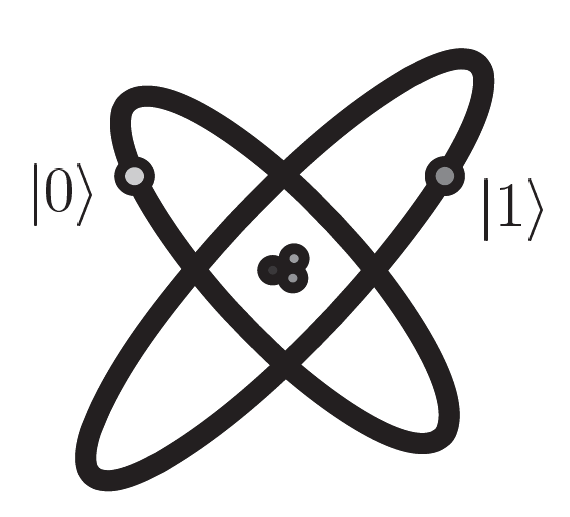
\includegraphics[scale=.4]{atom.png}
	\centering
	\caption{Qubit represented by two electron orbits in an atom, \cite{Nielsen2002}.}
	\label{fig 1.1}
\end{figure}


\section{Postulate 3: Evolution}


The third postulate of quantum mechanics modulates the evolution of a quantum system. That is, the evolution of the state vector that describes the system. In order to properly formalize it we need the concepts of eigenvector and eigenvalues, as well as the Hermitian operators.


\subsection{Eigenvalues and eigenvectors}


\begin{definition}
	Let $V$ be a vector space and $A$ an operator on $V$. An \emph{eigenvector} is a non zero vector $|v_\lambda\rangle$ such that $A|v_\lambda\rangle = \lambda|v_\lambda\rangle$ for a complex value $\lambda$ called the associated \emph{eigenvalue}.
\end{definition}

Eigenvalues and associated eigenvectors will usually be denoted with the same letter for simplicity: $\lambda$ and $|\lambda\rangle$. We assume the reader is familiar with eigenvectors and values basic notions. For instance, that they may be calculated using the \emph{characteristic equation}: $|I - \lambda A| = 0$.

\begin{definition}
	A \emph{diagonal representation} of an operator $A$ is a representation $\sum_i \lambda_i |\lambda_i\rangle\langle\lambda_i|$ where the $|\lambda_i\rangle$ form an orthonormal set of A's eigenvectors and $\lambda_i$ are the respective eigenvalues. An operator is said to be \emph{diagonalizable} if it allows a diagonal representation.
\end{definition}

\begin{exampleth}
	As an example of this, let us consider the following matrix:
	
	$$ Z = 
	\begin{pmatrix}
		1 & 0 \\
		0 & -1 
	\end{pmatrix}
	$$
	
	This matrix is called the \emph{Z Pauli} matrix. It is relevant for quantum computing and it will be introduced later on along with the rest of the Pauli matrices. For now, lets compute its diagonalizable representation. Since it is already diagonal we can infer that its eigenvalues are $\{1, -1\}$. Computing the diagonal representation we realize that a pair orthonormal eigenvectors are $\{|0\rangle, |1\rangle\}$ respectively. Therefore:
	
	$$ Z = 
	\begin{pmatrix}
		1 & 0 \\
		0 & -1 
	\end{pmatrix} = 
	|0\rangle\langle0| - |1\rangle\langle1|
	$$
\end{exampleth}

Normal operators have significant relevancy thanks to the following result:

\begin{theorem}[Spectral Decomposition Theorem]
	An operator $A$ is normal if and only if it is diagonalizable.
\end{theorem}
\begin{proof}
	TODO: To be copied, Box 2.2, page 72, Nielsenchen.
\end{proof}

Since Hermitian and unitary operators are normal, we obtain the following result:

\begin{corollary}
	Any Hermitian operator is diagonalizable. Any unitary operator is diagonalizable.
\end{corollary}


\subsection{Postulate 3 statement}


\begin{postulate}
	The evolution of a \emph{closed} quantum system is described by a\emph{unitary transformation}. That is, the state $|\varphi\rangle$ of the system at time $t_1$ is related to the state $|\varphi'\rangle$ of the system at time $t_2$ by a unitary operator $U$ which depends only on the times $t_1$ and $t_2$,
	
	$$ |\varphi'\rangle = U|\varphi\rangle $$
\end{postulate}

It is worth mentioning that this postulated assumes our physical system to be \emph{isolated}. That is, there is no interaction with the system coming from the exterior. In reality, the only real closed system is the universe as a whole. However, we can recreate sufficiently closed systems so that they can be described with approximations as being closed. 

Just like the first postulate does not provide the state space or state vector of the system, the second postulate does not provide the unitary transformation that concretes this evolution. For our quantum computing case, we will be the ones to define the unitary transformation applied to the system. That is, the quantum circuit that transforms our qubit.

The description of the system evolution provided by \ref{postulate 2} only provides information for those fixed times $t_1$ and $t_2$. A continuous time description of this evolution is provided by the Schrodinger equation, which provides a redefinition of the second postulate.

\begin{postulate}
	The time evolution of the state of a \emph{closed} quantum system is described by the Schrodinger equation:
	
	$$ i \hbar \frac{d|\varphi\rangle}{dt} = H|\varphi\rangle $$
	
	where $\hbar$ is \emph{Planck’s constant}, $i$ is the imaginary unit and $H$ is a fixed Hermitian operator known as the $Hamiltonian$.
\end{postulate}

There are several notes to make about this postulate. First, the Hamiltonian is fixed for the given system and it is not be confused with the \emph{Hadamard quantum gate}, also represented by an $H$. Second, $\hbar$ is a physical constant that can be absorbed into the Hamiltonian for our purposes, simplifying the equation. Finally, this is a differential equation, so by knowing the initial state space of the system and the exact Hamiltonian we may know the exact evolution of the system.

Lets study the Hamiltonian in general. Since it is a Hermitian operator, it allows a spectral decomposition by the spectral decomposition theorem (TODOref Spectral Decomposition theorem):

$$ H = \sum_E E |E\rangle\langle E| $$

where $E$ are the eigenvalues and $|E\rangle$ the respective eigenvectors. 


TODO: O bien aquí o bien en otro sitio, comentar el ejemplo de Manzano sobre medidas respecto de los estados energéticos


\subsection{Quantum Computing perspective: ?}

In practice, obtaining the Hamiltonian for a given quantum system is a really laborious work and usually needs experimental data (TODO: add evidence? stated as such in Niel.). However, for our computational purposes we will be the ones designing the Hamiltonian such that our system evolves as desired. In particular, chapter 3 (TODO: add ref to QUBO chapter) describes in detail the construction of Hamiltonians for QUBO problems.

TODO: Completar



\section{Postulate 4: Composite systems}

\subsection{Tensor product}

\subsection{Postulate 4 statement}


\subsection{Quantum Computing perspective: Multiple qubits}


Suppose we have a pair of qubits. In the classical case, two bits can be in four possible states: 00, 01, 10, and 11. Similarly, the two qubits computational basis states are $|00\rangle$, $|01\rangle$, $|10\rangle$ and $|11\rangle$. Just like in the single qubit case, our two qubits system may be in a superposition of these four states:

$$ |\varphi\rangle = \alpha_{00} |00\rangle + \alpha_{01} |01\rangle + \alpha_{10} |10\rangle + \alpha_{11} |11\rangle $$

Correspondingly, the measurement of this system will result in either 00, 01, 10 or 11. In fact, it will yield state $x$ with probability $|\alpha_x|^2$, being $\alpha_x$ the coefficient associated with the state $|x\rangle$. The condition of the probabilities adding up to one is called the \emph{normalization condition} and can be expressed as $\sum_{x \in \{0,1\}^2} |\alpha_x|^2 = 1$ for the two qubits case, where $\{0,1\}^2$ are the strings of length two where each character is either $0$ or $1$.

The fundamental differences with the single qubit case start on measurement. Of course, we can measure both qubits at the same time, but we could also measure only one of them. Upon measuring the first qubit we would obtain $0$ with probability $p_0 = |\alpha_{00}|^2 + |\alpha_{01}|^2$, since these are the coefficients associated with the first qubit being $0$. Furthermore, our system will collapse to:

$$ |\varphi'\rangle = \frac{ \alpha_{00} |00\rangle +f \alpha_{01} |01\rangle }{ \sqrt{|\alpha_{00}|^2 + |\alpha_{01}|^2} } $$

Note the normalization term $\sqrt{|\alpha_{00}|^2 + |\alpha_{01}|^2}$, applied so the post-measurement state still satisfies the normalization condition. Naturally, after obtaining $0$ in the first qubit we can still obtain either $0$ or $1$ in the second qubit, with probabilities 

$$ \frac{ |\alpha_{00}|^2 }{ |\alpha_{00}|^2 + |\alpha_{01}|^2 }  \ \text{ and } \ 
\frac{ |\alpha_{01}|^2 }{ |\alpha_{00}|^2 + |\alpha_{01}|^2 } $$

respectively, adding up to $1$. Correspondingly, the first qubit being measured will yield $1$ with probability $p_1 = |\alpha_{10}|^2 + |\alpha_{11}|^2$.

Additionally, the first qubit independently should satisfy the normalization condition. That is, its probabilities of being $0$ and $1$ upon measurement must add up to $1$. But those are $p_0$ and $p_1$, which add up to one because of the normalization condition for $|\varphi\rangle$, as expected.

We now introduce the \emph{Bell State} or \emph{EPR pair:}

$$ \frac{ |00\rangle + |11\rangle }{ \sqrt 2 } $$

Although it may seem harmless at first glance, this state has been responsible for many surprises during the development of quantum physics [TODOref to the EPR paradox]. Let us have a first look into it, although we will come back to it in section [TODOref la seccion dodne comentamos el problema de la teletransportación cuántica].

Upon measuring this system we may obtain state $|00\rangle$ with probability $1/2$ and state $|11\rangle$ with probability $1/2$. Suppose we measure the first qubit and obtain $0$. Then, the second qubit will always yield $0$ upon measurement. This means both outcomes are \emph{correlated}. This fact is known as \textbf{quantum entanglement}. It rests at the heart of the disparity between classic physics and quantum physics. It was deeply studied first by Einstein, Podolsky, and Rosen (EPR) \cite{Einstein1935} and second by John Bell \cite{Bellt1964}.

Let us finally consider the more general case. In an n-qubits system our computational basis would consist of the sates $|x_1 x_2 \dotsc x_n\rangle$, where $x_i \in \{0,1\}$. As we already know, in a single qubit system we have two amplitudes $\alpha_0$ and $\alpha_1$. We have four amplitudes for a 2-qubits system, eight for a 3-qubits system... And $2^n$ for an n-qubits system. This means that the number of amplitudes grows exponentially as we add qubits to the system. An immense increment concerning the classical case was the quantity of information that our simple holds grows linearly with the numbers of bits. Of course, we already know it is not that simple, since there are huge limitations on how we may access this information in the quantum realm such as how a qubit collapses upon measurement and the non-cloning theorem discussed in section [TODO]. But we can already glimpse the power of quantum computing versus the classical one.




% Part II
%\ctparttext{
	\color{black}
	\begin{center}
		TODO: cambiar la descripción de la parte (antes del titulo)
	\end{center}
}

\part{Parte de matemáticas}

\chapter{The Genome Assembly Problem}

The genome of an organism is all its genetic material \cite{Roth2019}. The deoxyribonucleic acid (DNA) is the carrier of that genetic information. It consists of two long chains twisted to form a double helix \cite{Alberts2007}. Each of these chains is composed of a series of nucleotides or bases: adenine (A), guanine (G), cytosine (C), and thymine (T). Since these bases are matched in pairs in the DNA double helix, those are called base pairs (bp).

A genome sequence is the complete list of nucleotides of every chromosome of an organism. With today's technology, automated sequence machines can read up to 1000 bp at a time \cite{Slatko2011} while the human genome contains 3 Mbp, so we can't just read the whole genome. This is where genome assembly comes in.

Genome assembly refers to the process of, given a large number of short DNA reads, stitch them together to form a large representation of the original chromosome where the reads came from. The two main techniques used to reconstruct these sequences are the ab initio reference-free alignment and the de novo reference-based assembly.

\section{Ab initio reference-based alignment}

In this method, the DNA reads are matched against a known trusted reference of the same organism. This is essentially a pattern matching problem, where we find the index of a given sub-string in a larger string. However, after the reconstruction is complete the result is compared to the reference in order to identify implications; therefore introducing bias based on the reference \cite{Sarkar2020}.

In the naive approach, the short sub-string is compared to the reference starting at the first index. If the end of the sub-string is reached with a positive, a match is obtained. Otherwise, the sub-string is shifted a single position and we compare again. Heuristic methods that improve on this idea are based on shifting a greater number of spaces after a mismatch.

Different number of strategies have been developed in this direction. For instance, the classic Boyer-Moore and Knuth-Pratt-Morris algorithms \cite{Holmes1999}. However, these in particular are not adequate for genome assembly since these are exact string matching algorithms and DNA reads usually need approximate matches due to reads errors. Other algorithms worth mentioning are the Needleman-Wunsch algorithm \cite{Needleman1970} and the Smith-Waterman algorithm \cite{Smith1981}, for global and local alignment respectively. These are dynamic programming algorithms designed specifically with DNA reads in mind. 

State of the art algorithms trades off accuracy for speed and memory. The approximation and errors introduced prevents the application of this technique to critical areas such as personalized medicine. Given enough computational power, the de novo method yields better results.

\section{De novo reference-free assembly}

This method is reference-free, being based only on DNA reads. Thus, it has no reference bias but it is more computationally complex. It is usually used the first time a species DNA is read.

In this technique, multiple copies of the same DNA are made before slicing it. After chopping each copy at random places the data is redundant and the different reads overlap, making the assembly easier.
























% ----------------------- %
% BIBLIOGRAFÍA
% ----------------------- %

% Estilo de cita.
\bibliographystyle{unsrtnat}

%[citestyle=numeric]

% Añadimos la bibliografía al índice
\phantomsection
\addcontentsline{toc}{chapter}{Bibliography}

\bibliography{bib/library.bib}

\end{document}